\documentclass[../main.tex]{subfiles}
\begin{document}

\chapter{Securing the communication channel}
\emph{Using HTTPS in combination with Strict Transport Security is the baseline for building secure
web applications.}

\section{Introduction}
\subsection{Towards secure communication}
\begin{itemize}
\item The correct use of \textbf{HTTPS} prevents many network-based attacks and helps keep your users safe.
\end{itemize}

\subsection{The dangers of an unprotected channel}
\begin{itemize}
\item To attack a \textbf{wireless network} you just have to be nearby, in stead of have physical access to the cable.
\item when you visit a website using HTTPS, the HTTPS protocol makes sure you are talking to this website and nothing else. You are sure that you are communicating to the website that you want and on top of that it, also encrypts your traffic. No one can see what you are sending and it also authenticates your traffic, which basically means that no one can modify data or inject content into a web page. 
\item You are connected to an open network, if you then use HTTPS to, for example, log into a website or send your credit card information, an attacker would not be able to attack you, because HTTPS takes care of all the security risks.
\end{itemize}

\subsection{The recent push for HTTPS}
\begin{itemize}
\item After the NSA leaks by Edward Snowden, the whole web started a shift to HTTPS (Google prioritized HTTPS search results, major companies launched initiatives to increase the use of HTTPS, \textbf{let's encrypt} founded,...).
\item Browsers implemented numerous features to push the use of HTTPS (access microphone/webcam requires secure connection, mark login forms using normal HTTP as insecure,...)
\item An HTTPS pages embedded in an HTTP page (or opened as a pop-up from an HTTP page) is not seen as secure in modern browsers.
\item Although the shift to HTTP started slowly, the number of HTTPS deployments is booming right now.
\item The \textbf{quality of the secure connection} depends on the strengths of the individual configuration options. You can test the quality of any website with the \textbf{Qualys SSL Server Test}.
\item The \textbf{SSL Pulse project} uses the SSL Server Test to automate the scanning of popular sites every month and keeps track of the results.
\item 13,0\% (2015) $\rightarrow$ 59,1\% (2017) HTTPS deployements (massive improvement)
\end{itemize}

\section{Underpinnings of HTTPS}
\subsection{Security properties of HTTPS}
\begin{itemize}
\item On the highest level, HTTP and HTTPS are the same protocol. The difference is that with HTTPS, an additional protocol is added to the network stack:  \textbf{SSL}, which stands for \textbf{Secure Sockets Layer} or \textbf{TLS}, which stands for \textbf{Transport Layer Security}. (Actually TLS is the successor of SSL)
\item With normal insecure HTTP traffic, the message traverses the network stack. In each layer of the network stack, extra information is added to the packet. The contents of the message are transmitted in plain text.
\begin{figure}[h!]
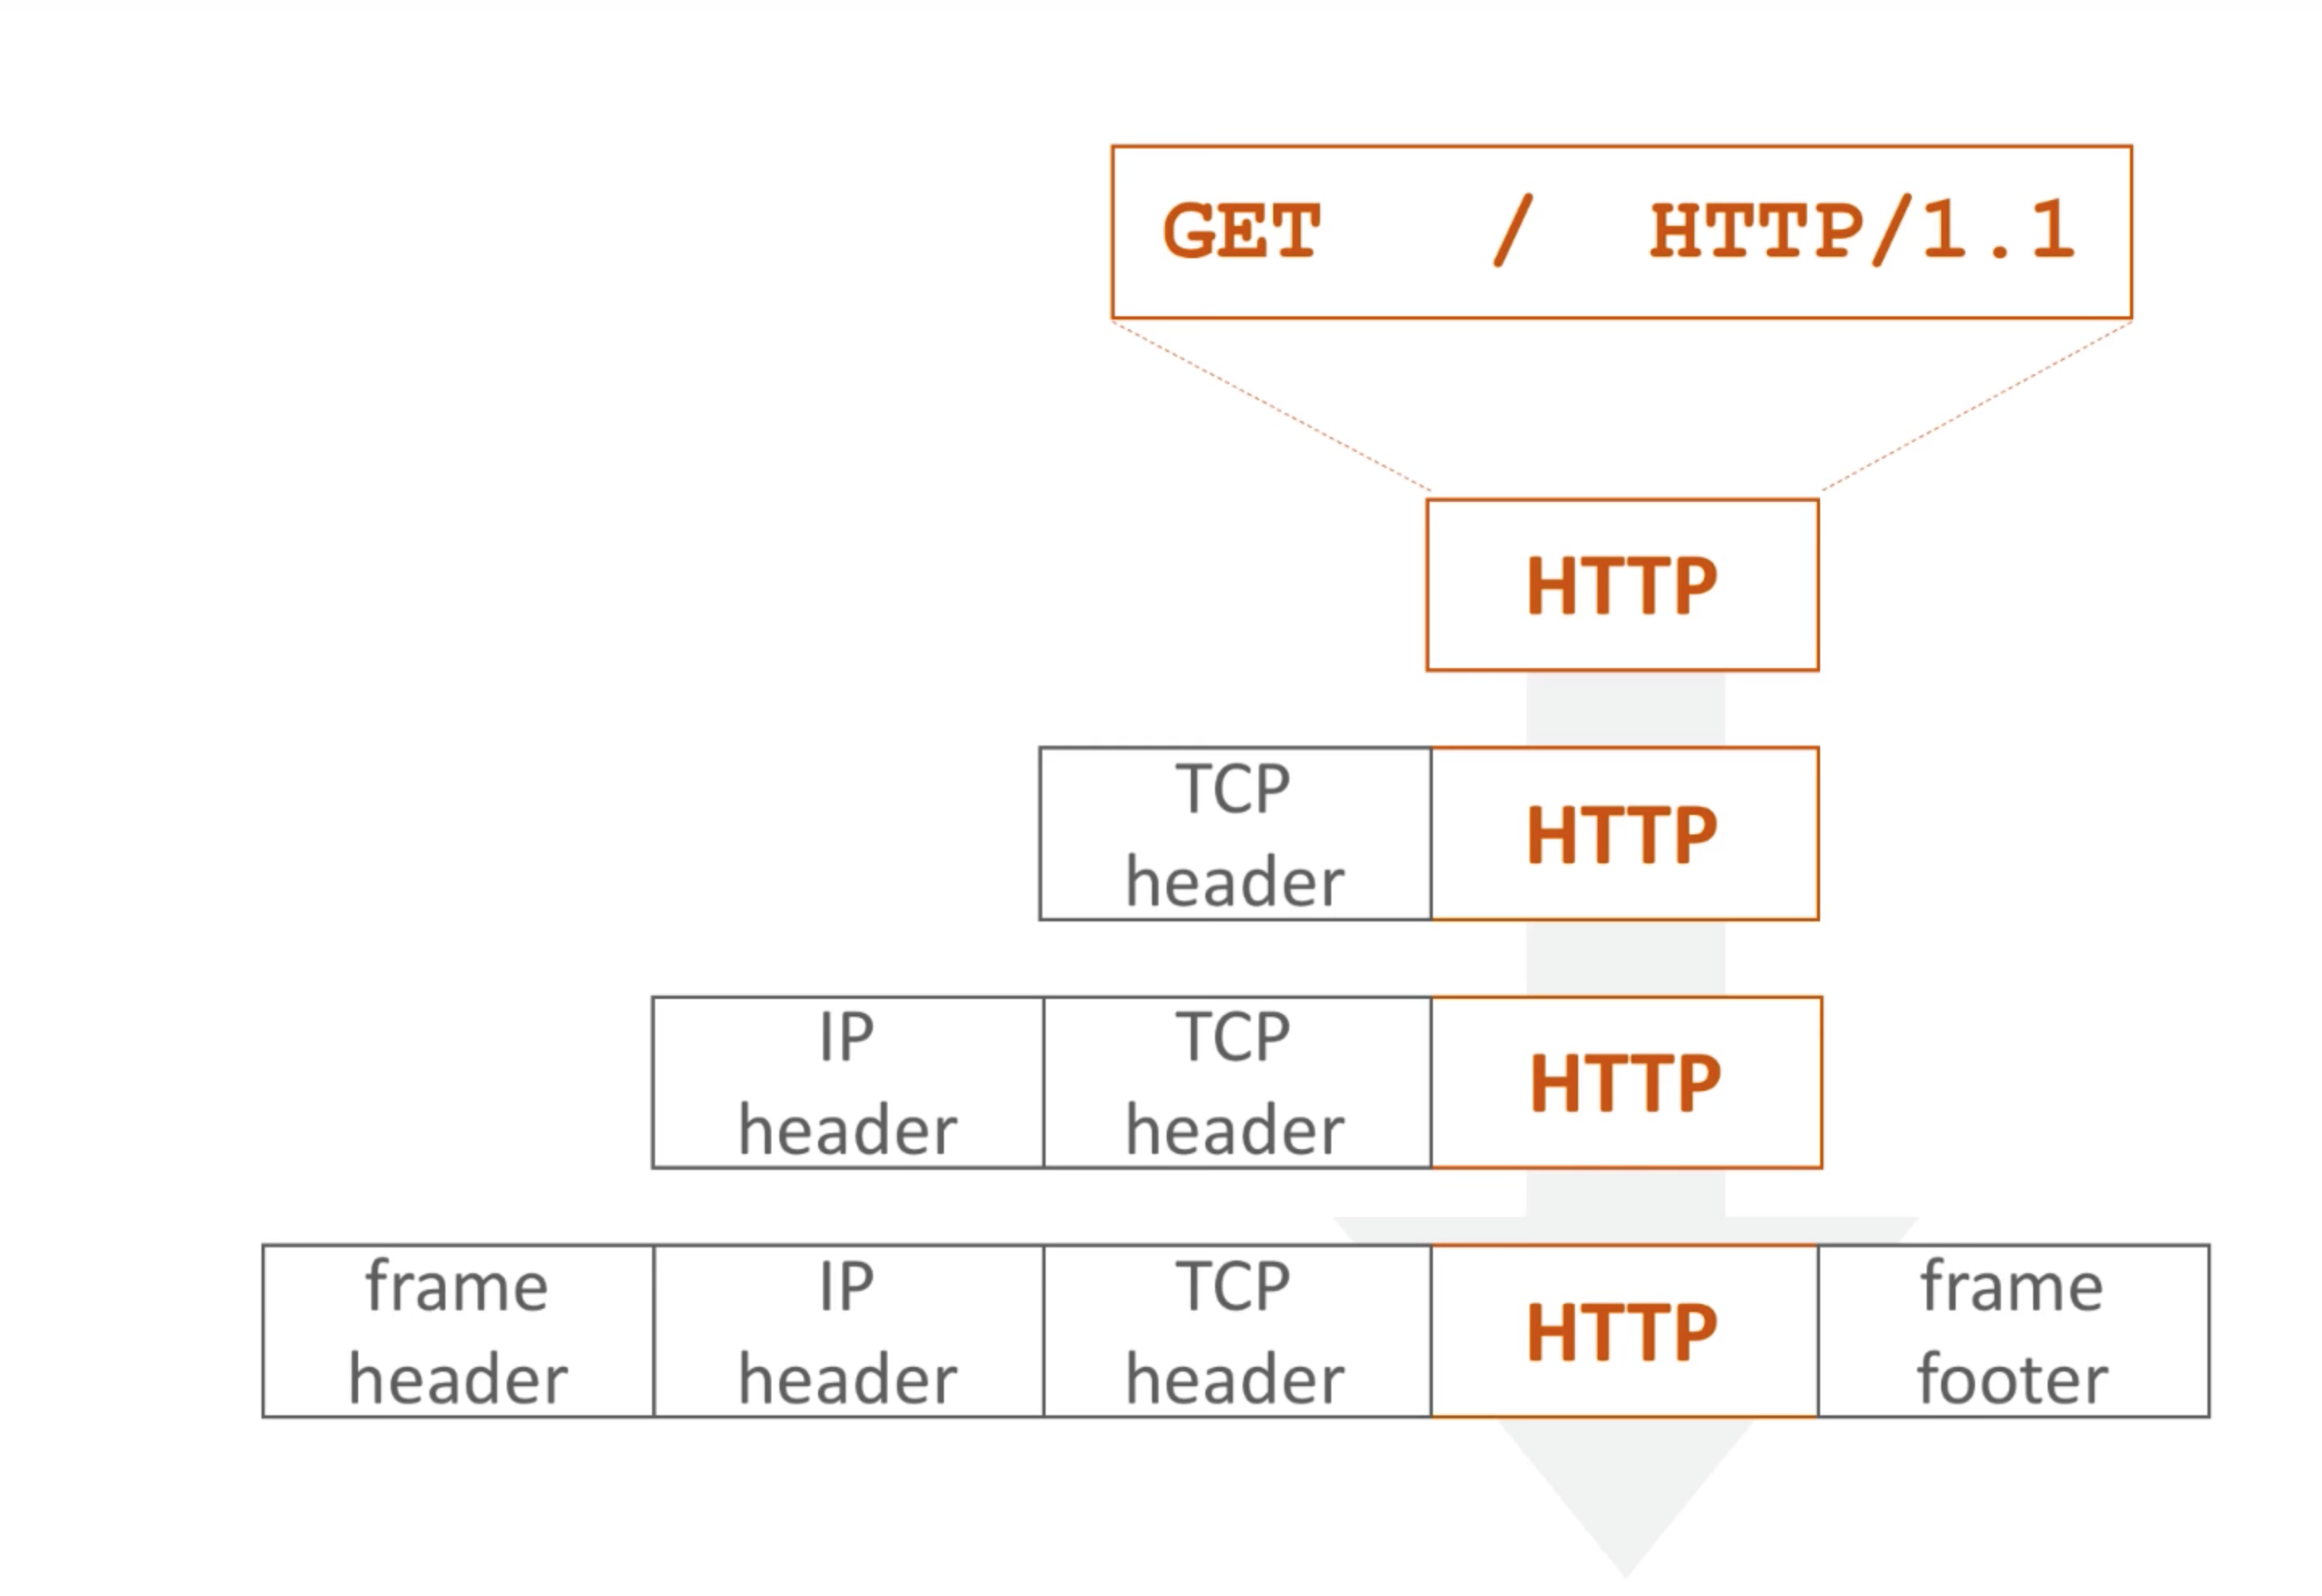
\includegraphics[width=\textwidth]{../images/http}
\caption{Http message traversing through the network stack, adding information}
\end{figure}
\item With HTTPS, the network stack incorporates the TLS protocol (between application and transport layer). It encapsulates the HTTP message and ensures confidentiality and integrity. The TLS record is then passed along the network stack.
\begin{figure}[h!]
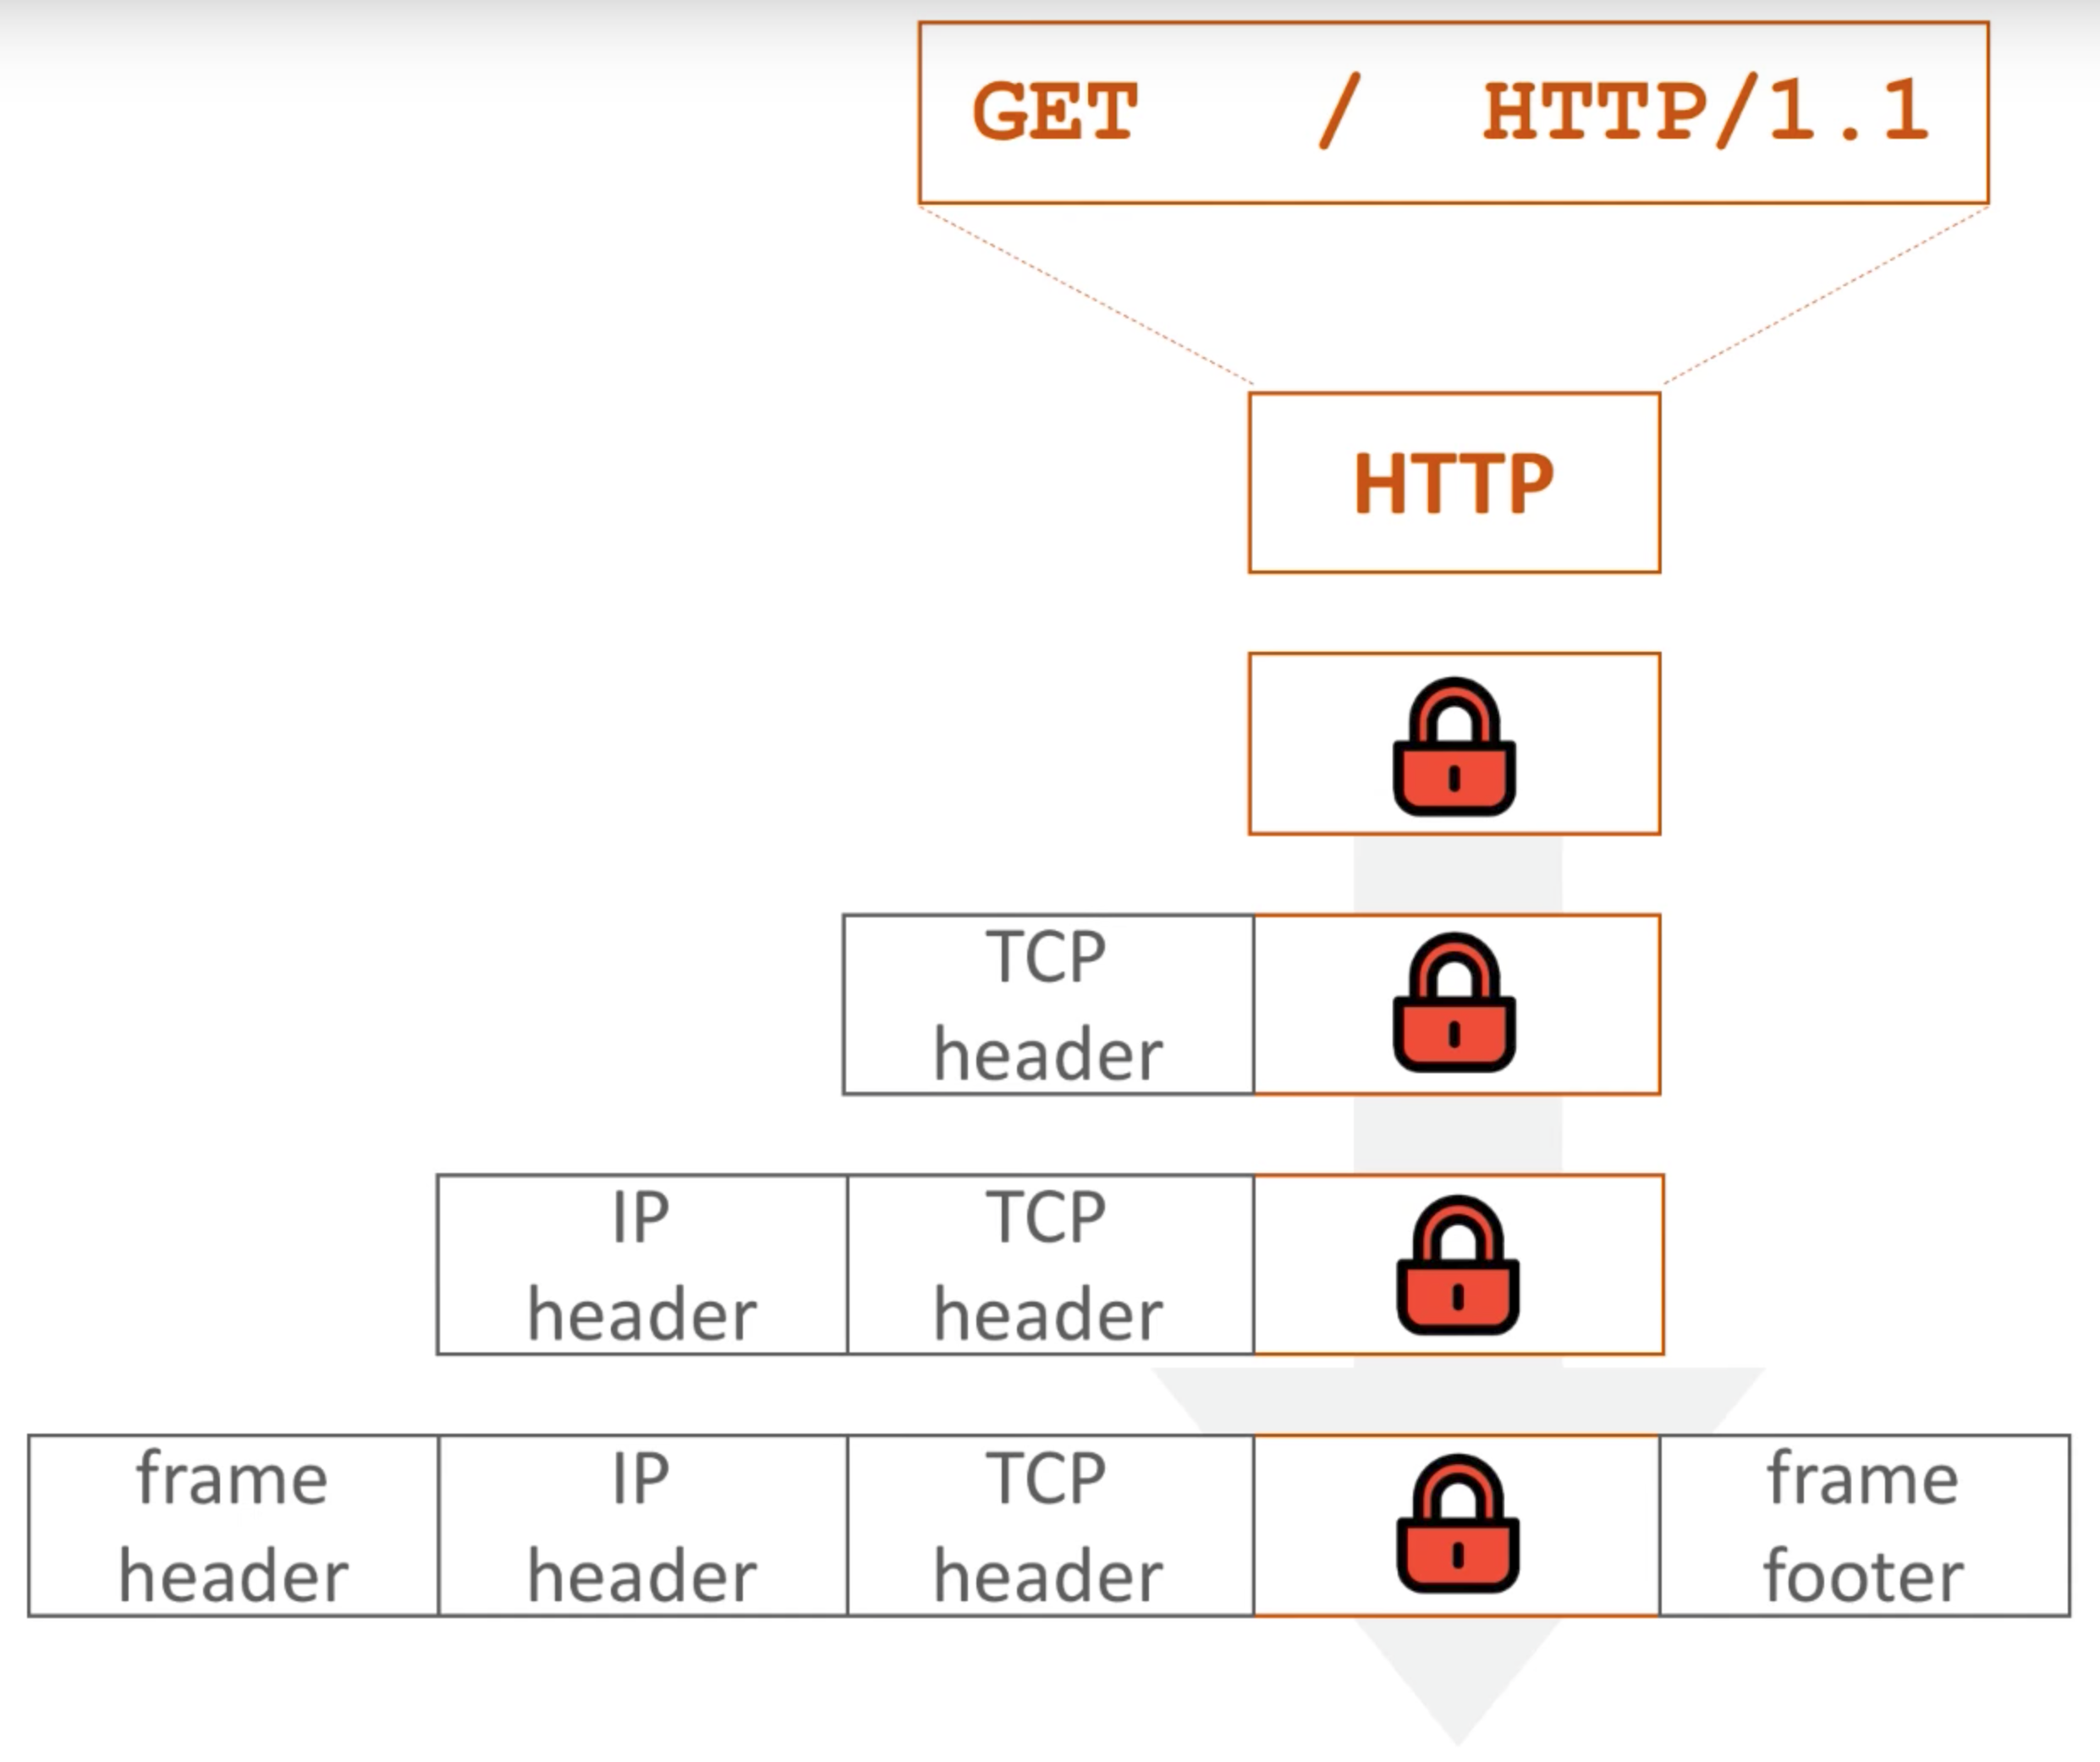
\includegraphics[width=\textwidth]{../images/https}
\caption{Http message traversing through the network stack, adding information}
\end{figure}
\item This way, the HTTP message is replaced by encrypted data.
\item Because of the layered design, the TLS protocol is suitable for other protocols as well (POP, SMTP, IMAP,...).
\item Security properties of SSL/TLS
\begin{enumerate}
\item \textbf{Confidentiality:} ensures that unauthorized parties cannot read the data transmitted over the network.
\item \textbf{Integrity:} ensures that when the data is tampered with, the receiver can detect this.
\item \textbf{Authenticity:} ensures that an attacker cannot get a man in the middle position.
\begin{itemize}
\item \textbf{Record protocol:} ensures the confidentiality and integrity of the transmitted data.
\item \textbf{Handshake protocol:} handles establishing a new connection and ensures authenticity before establishing a secure channel (browser verifies the identity of the server). This step is crucial to avoid \textbf{man in the middle attacks}, where the attacker impersonates a legitimate server. A successful impersonation attack renders confidentiality and integrity useless. The messages of the handshake protocol are sent in plain text. This is not a real problem since these messages do not contain sensitive information.
\end{itemize}
\end{enumerate}
\item The Handshake protocol and Record protocol are \textbf{sub-protocols} of TLS.
\item In essence, an attacker on the network cannot read messages, manipulate any messages, or impersonate a legitimate server without detection.
\item The browser takes authenticity problems very seriously. It will not establish a connection to the server and show a big scary warning page to the user instead, explaining the problem.
\item A few \textbf{limitations} to the power of TLS.
\begin{enumerate}
\item An attacker can \textbf{still observe the communication}. From the network data, the attacker can derive which server you are connecting to, so TLS does not ensure privacy about the communication.
\item Even encrypted messages are subject to traffic analysis techniques. Researchers have shown that traffic analysis of encrypted data can leak information about the unencrypted contents. They illustrated their approach on the video streams sent by Netflix. By analyzing the amount of data sent in the HTTPS stream, they could determine which stream
was being watched.
\end{enumerate}
\item The benefits of HTTPS are crucial in the modern web. Under no circumstances are the limitations we discussed here an argument to abstain from deploying HTTPS.
\end{itemize}

\subsection{Keys, certificates and ciphers}
\begin{itemize}
\item Each version of the TLS specification introduces new \textbf{cryptographic algorithms}. These algorithms are essential to achieving the security properties of HTTPS. The browser and server negotiate which algorithms they will use during the handshake. Each algorithm serves a particular purpose, and the combination is referred to as a \textbf{cipher suite}.
\item Confidentiality is achieved using a symmetric-key algorithm. Such an algorithm encrypts the message using a specific key. Since the algorithm is symmetric, decrypting the message only works with the same key. For HTTPS, this means that both the browser and the server need to use the same shared key.
\item In TLS, integrity comes from using an \textbf{HMAC function}. Such a function uses a secret key to calculate a checksum for a specific message. To verify a checksum, the receiver recalculates the checksum on the received message using the same key. By comparing both checksums, the receiver can be sure that the message has not been tampered with.
\item Note that integrity does not prevent tampering, but ensures that tampering is detectable.
\item Both confidentiality and integrity depend on the use of secret keys. In TLS, these keys come from a cryptographic secret called the \textbf{pre-master secret}. Note that both browser and server need to have access to the same keys, hence the same pre-master secret. That is why the handshake contains a step called the \textbf{key exchange}, where browser and server share this pre-master secret. Exchanging such a secret over the network is harder than you might think. The key exchange takes place during the handshake, but at the time, a secure channel is not yet available.
\item Challenges for both parties on an untrusted network.
\begin{itemize}
\item Exchanging the pre-master secret in plain text exposes it to an eavesdropper. With the pre-master secret, the attacker is capable of breaking confidentiality and integrity. In TLS, we can use \textbf{asymmetric-key algorithms} to send the pre-master secret in a secure way: Use a key pair, that consists of a private and a public key. As the name indicates, the private key belongs to the owner, while the public key can be shared. Messages encrypted with the public key can be decrypted with the private key and vice versa.
\item The browser encrypts the pre-master secret with the \textbf{public key} of the server. So only the holder of the \textbf{private key} will be able to decrypt the message. Protecting the pre-master secret this way suffices to ensure confidentiality and integrity.
\item For this to work, the browser needs get the server’s public key. Knowing all the keys for all the websites up front is not very practical. That’s why the server sends the browser his public key during one of the first steps of the TLS handshake.
\item Of course, we need extra security measures to prevent man in the middle attacks. This is achieved by the third security property of TLS: authenticity. Within the TLS protocol, authenticity is ensured using \textbf{certificates}. A certificate associates a specific public key, and hence the associated private key, with a specific domain. During the handshake, the server sends his public key along with the certificate. The browser verifies the validity of the certificate and checks if the domain matches the certificate. If everything succeeds, the browser knows that he is talking to a legitimate server. The pre-master secret can now be exchanged using the public key of the server. Once the handshake is completed, the secure channel can be established.
\item The introduction of certificates has \textbf{completely redefined the problem}, the security of an HTTPS connection now depends entirely on the authenticity property. Only a legitimate server can present a valid certificate, and only that server knows the
corresponding private key. To impersonate a legitimate server, the attacker needs a valid certificate and the associated key pair.
\end{itemize}
\end{itemize}

\subsection{Common misconceptions about HTTPS}
\begin{enumerate}
\item \emph{HTTPS is only relevant for sensitive content, such as login forms or online payments.}\\[0.2cm]
This is no longer true. The moment your application sends an HTTP request, your users become vulnerable to a
variety of attacks.
\item \emph{HTTPS has a significant performance impact, and your servers will not be able to handle it.}\\[0.2cm]
Modern CPUs come with support for AES, the encryption algorithm used in almost all HTTPS
deployments. On top of that, the TLS protocol has undergone significant performance tuning. The performance aspect of HTTPS has long been the primary argument to weasel out of security obligations.\\[0.2cm]
e.g. Netflix has been running all their streaming services over HTTPS for quite some time. And to be clear, Netflix accounts for more than one-third of traffic during peak hours in the US.
\item \emph{Certificates are expensive, and a nightmare to configure.}\\[0.2cm]
Today, services like \textbf{Let’s Encrypt} offer free certificates for everyone. Let’s Encrypt even provides you with the tool support to automate the whole process. One command takes care of requesting, installing and renewing certificates. This makes setting up HTTPS a five-minute job.
\item \emph{You can only run one HTTPS application per IP address.}\\[0.2cm]
Today, almost every client supports a TLS extension called \textbf{Server Name Indication}, or \textbf{SNI} in short.
\end{enumerate}
$\Rightarrow$ There is almost no valid excuse to hold off on deploying HTTPS.
\clearpage

\section{Deploying HTTPS}
\subsection{Perfect Forward Secrecy}
\begin{itemize}
\item In a classic HTTPS deployment the browser sends the encrypted secret over an insecure channel. Even if someone is listening, only the legitimate server can decrypt the secret. 
Disadvantage $\rightarrow$ It cannot guarantee confidentiality towards the future.\\
Imagine an attacker who records an entire HTTPS conversation, including the handshake. If the attacker comes in possession of the server's private key in the future, he can decrypt the pre-master secret. Having this secret enables the attacker to derive the shared keys, and decrypt the entire conversation.
\item Nobody thought this was relevant until the Snowden leaks.
\item Solution $\rightarrow$ deploy a key exchange algorithm that supports perfect forward secrecy: \textbf{Diffie-Hellman} key exchange algorithm.
\item Simplified explanation:\\
Alice and Bob need to establish a shared secret, represented by a color of paint. First, they decide to start with a shared color, yellow. Note that this fact does not need to be kept a secret. Next, they both choose their secret color and mix it into the starting color. They exchange their mixed bucket of paint over an insecure channel. Now, they both add their secret color into the mixtures. They both end up with the same shared secret color. In this example, the truck driver can see that Alice and Bob exchanged a bucket of green and orange. He also knows that they started out with yellow, but there is no way to combine those three colors into the same brown color that both Alice and Bob have. This looks easy to solve, but is is a hard mathematical problem.
\item In the actual Diffie-Hellman algorithm, separating colors means solving the \textbf{discrete logarithm problem}.
\item To increase the security of the algorithm, you should choose new private parameters, or private colors, for each connection (=\textbf{ephemeral Diffie-Hellman}).
\item The plain Diffie-Hellman algorithm is vulnerable to man in the middle attacks $\rightarrow$ combined with an asymmetric key algorithm. In practice, the server generates a digital signature with its private key, and the browser verifies it with the server's public key.
\item \textbf{Perfect forward secrecy} ensures the use of a new key for every connection. It also ensures that this key is not encrypted with the server's public key, so it cannot be decrypted later. As a result, a captured session remains secure, even if the server's key is compromised in the future.
\end{itemize}
$\Rightarrow$ Perfect forward secrecy is a desirable property for all encrypted communication $\rightarrow$ all modern HTTPS deployments should use the Diffie-Hellman key exchange.

\subsection{Finetuning HTTPS for security}
\begin{itemize}
\item All new versions introduced stronger algorithms and better security features. As a consequence, a default TLS configuration requires a bit of fine-tuning to ensure an optimal security level.
\item Today, the most relevant versions ok SSL/TLS are SSL 3, TLS 1.0, TLS 1.1 and TLS 1.2.
\item SSL 3 is considered broken, but the others are still considered secure.
\item Why not disable all versions but the latest and most secure one? $\rightarrow$ client support.
\item It's about finding a balance between security and client support.
\item Even TLS versions that are considered secure contain insecure algorithms $\rightarrow$ handpick a set of secure algorithms. Again, the selection of algorithms is driven by balancing security and client support.
\item One of the biggest challenges in deploying TLS is figuring out if your configuration is secure $\rightarrow$  Qualys SSL Server Test (also gives you an overview of client connectivity).
\item For local development use \textbf{testssl.sh}.
\end{itemize}
\clearpage

\section{HTTPS in your application}
\subsection{Dealing with mixed content}
\begin{itemize}
\item \textbf{Mixed content blocking:} browser protects a secure page by refusing to load scripts and styles over an insecure HTTP connection. The moment we start loading resources over HTTP, the security guarantees of HTTPS no longer hold.
\item Initially, the browsers only displayed warnings about mixed content.
\item Modern browsers today make a distinction between passive and active mixed content.
\item \textbf{Passive mixed content:}  content that is only displayed, and thus only pose a limited threat (e.g. images, audio files, and video files). It is still loaded, but the developer sees a warning.
\item \textbf{Active mixed content:} has full access to the page, and thus poses a significant risk (e.g. scripts, styles, iframes, and objects). Because of its dangerous nature, the browser blocks active mixed content.
\item Transitioning to HTTPS can be harder than you think. The best piece of advice in there is to take it slow. Perform the transition to HTTPS gradually, and learn how to deal with problems along the way.
\item You need to get an idea of the size of your mixed content problem before addressing it $\rightarrow$ Content Security Policy.
\item \textbf{Content Security Policy (CSP):} security policy that allows you to control what content can be loaded on your pages. The server gives the browser a policy configuration that the browser enforces on the page. It has the capability to send reports when a given policy is violated. You can set up your own report-uri endpoint of use the freely available \textbf{report-uri.io} service.
\begin{figure}[h!]
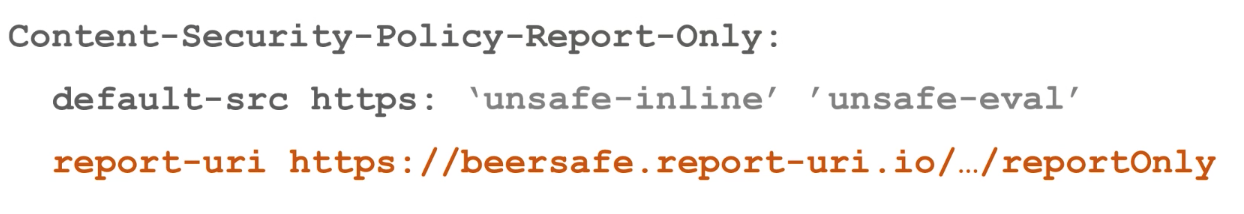
\includegraphics[width=\textwidth]{../images/csp}
\caption{Configuration of CSP to report non-HTTP traffic.}
\end{figure}
\item By running the application for some time with a CSP header enabled, we can extract a list of HTTP resources from the violation reports. If these HTTP resources contain active content, our application will break when we move to HTTPS.
\end{itemize}

\subsection{Partial HTTPS deployments are not the answer}
\begin{itemize}
\item Once you start deploying HTTPS in a real-life scenario, all kinds of questions will rise.
\item \emph{Can you run different HTTPS sites on one server?}
\begin{itemize}
\item Until a few years ago, you could only run one HTTPS application per IP address.
\item If the server hosts multiple HTTPS web applications, it needs to know which application the browser is connecting to.
\item If the server uses the wrong certificate, the browser will detect a mismatch between the domain of the certificate and that of the actual request. TLS handshake does not support sending the domain name of the application up front.
\item Modern browsers and operating systems support a TLS extension: \textbf{Server Name Indication}, or \textbf{SNI}.
\item With SNI enabled, the client includes the domain name of the application it is connecting to in the first step of the handshake. Now that the domain name is known up front, the server can select the right certificate. In this scenario, SNI is essential to establish the connection without errors.
\end{itemize}
\item \emph{Where do you store the sensitive cryptographic material?}
\begin{itemize}
\item Deploying a reverse proxy service as a dedicated TLS endpoint.
\item The proxy establishes the secure communication channel with a client. In the background, the proxy forwards all requests to internal services.
\item This setup can seem a bit strange but offers several benefits:
\begin{enumerate}
\item The deployment of internal services becomes a lot more practical. Now, they no longer need to worry about the public-facing TLS configuration.
\item It isolates the cryptographic material on a separate host or container. This isolation keeps the cryptographic material out of reach when an attacker targets the web application.
\end{enumerate}
\item Specialized companies are offering various traffic optimization services, including the configuration of HTTPS (e.g. \textbf{CloudFlare}).
\end{itemize}
\item \emph{What happens if you use a third-party service for traffic optimization?}
\begin{itemize}
\item Because an external service handles HTTPS, there is no secure end-to-end communication channel.
\item The service offering HTTPS support has a full man in the middle position, giving it full access to all traffic.
\item Using such a service means accepting the risk that there is another trusted party, which can become compromised or turn malicious.
\end{itemize}
\end{itemize}

\subsection{Redirecting HTTP to HTTPS}
\begin{itemize}
\item Turning off support for HTTP is a straightforward way to force the use of HTTPS. If the server no longer listens to HTTP traffic, connection attempts will result in an error. From a security perspective, this seems like a good idea. But from a usability perspective, this approach has a significant impact on your application.
\item All existing URLs that point to an HTTP page will stop working, but even for a new project the standard url construction of modern browsers uses HTTP.
\item We can use a redirect mechanism to send all traffic from the HTTP version of our application to the HTTPS version: 
\begin{enumerate}
\item The browser transforms this domain name into an HTTP request and sends it to the server.
\item But instead of serving the contents, the server instructs the browser to load the HTTPS version of the page (\textbf{redirect}).
\item The HTTP response from the server has \textbf{status code 301} and a \textbf{Location header}. The status code indicates that the requested resource has moved permanently and the location header contains the new URL for the resource.
\item When the browser follows the redirect, a secure channel will be established. The browser can now load the page over HTTPS.
\end{enumerate}
\item This setting ensures that existing URLs, which may include query parameters, remain intact.
\item \emph{Why browsers do not use HTTPS to send the first request?}
\begin{itemize}
\item Not all applications support HTTPS out of the box, so the first request over HTTPS may result in error.
\item Retrying over HTTP is a bad idea. If this was the default behavior, how can the browser tell the difference between a legitimate error and an attack?
\item An attacker on the network can always force an error on the HTTPS request to trigger a downgrade to HTTP.
\end{itemize}
\item New security policy that you can use to further improve your HTTPS deployment: \textbf{Strict Transport Security}.
\end{itemize}

\subsection{Enabling Strict Transport Security}
\begin{itemize}
\item Unfortunately, the redirect to HTTPS itself remains vulnerable to network-based attacks.
\item By executing an \textbf{SSL stripping attack}, the attacker can get a man in the middle position: the attacker intercepts the HTTP request and prevents the redirect from happening. Instead, the attacker fetches the HTTPS page and serves it over HTTP.
\item The only way to stop SSL stripping attacks is by deploying additional security policies: \textbf{HTTP Strict Transport Security policy (HSTS)}.
\item With HSTS, a web application instructs the browser to use HTTPS by default for a specified period.
\item The server can configure an HSTS policy by sending a response header. The name of the header is “Strict-Transport-Security”, and it supports two configuration parameters. 
\item The first parameter, \textbf{max-age}, is mandatory and specifies the lifetime of the policy in seconds.
\item Note that the period is extended every time the browser sees this HSTS response header.
\item The second parameter of an HSTS policy is the optional \textbf{includeSubdomains flag}. This flag instructs the browser to apply the HSTS policy to all subdomains of the domain that sets the policy.
\item \emph{But what happens the very first time the user visits our application?}
\begin{itemize}
\item The first request is still sent over HTTP because this is the default browser behavior.
\item This means that if we visit an application for the first time over an insecure network, we are still vulnerable to an SSL stripping attack (\textbf{trust on first use problem}).
\item Inform the browser up front that the application wants to use HTTPS. For HSTS, browsers support a preload list of sites that want this type of behavior. Adding your site to the list of HSTS preloaded domains means opting into the mandatory use of HTTPS for all requests, even the very first one.
\item Before you can add yourself to the list, you need to meet several requirements (\textbf{hstspreload.org}).
\end{itemize}
\item If you want to disable your current policy, the max-age needs to be set to 0. Omitting the header from the response is insufficient to disable the policy.
\end{itemize}
\clearpage

\section{Advanced topics}
\subsection{Analyzing the trust model behind HTTPS}
\begin{itemize}
\item Earlier, we explained authenticity as verifying the validity of a certificate. While technically correct, we did omit the details about issuing and verifying a certificate.
\item Certificates are issued by a \textbf{Certificate Authority (CA)}. 
\item When the CA issues a new certificate, it signs the certificate using its private key. The browser can verify a certificate by using the CA’s public key to verify the signature. If it matches, the browser knows that the certificate is issued by the CA, and decides to trust it.
\item \emph{How can the browser know whether a key belongs to a CA or not?}
\begin{itemize}
\item The system works with different levels of CAs.
\item A CA signing end user certificates is an \textbf{intermediate CA}. An intermediate CA, in turn, needs a certificate from a higher-level CA to prove the legitimacy of its key material. This process can continue for a few steps until it reaches the highest level. At this level, we find CAs known as \textbf{root CA}s.
\item Every browser and operating system has a list of hardcoded root CAs
\item Whenever the browser needs to verify a certificate, it will verify every certificate in the chain, until it reaches a trusted root CA.
\end{itemize}
\item A browser only trusts certificates with a valid signature chain, on the condition that the other properties are also valid. These properties include, among others, a domain name, a start date, and an expiration date. All the properties of a certificate are added when the CA generates and signs the certificate.
\item Since the CA issues a certificate for a particular domain name, it implies that it should only
respond to legitimate requests.
\item \emph{How can a CA verify whether a request for a certificate is legitimate?}
\begin{itemize}
\item Verify whether the requester is in control of the domain for which the certificate is being requested.
\item One way to verify this is by sending a code to a reserved email address, such as postmaster@example.com. Only the legitimate owner can access such an email address. Another way would be to request that a particular response is placed at a specific location on the web server. Again, this is something that only an administrator can do, as it requires full access to the web server
\item These types of validation are what we call \textbf{domain validation} $\rightarrow$ cheapest and most common certificates.
\item CAs also offer certificates with \textbf{organization validation} and \textbf{extended validation}. For these types of validation, the CA performs more rigorous checks than verifying domain ownership. In return, these types of certificates are more expensive as well. For certificates with organization validation, there is no defined set of verification guidelines. For extended validation certificates, there is such a set.
\item On a cryptographic level, the type of validation does not impact the security of the connection. So is there an advantage of spending more money on a certificate, only to get stricter verification procedures? $\rightarrow$ Yes, the biggest difference is the browser UI. For extended validation certificates, the browser shows more information in the address bar.
\end{itemize}
\end{itemize}

\subsection{The fragility of the certificate ecosystem}
\begin{itemize}
\item Biggest problem concerning the certificate ecosystem: unconditional trust in root CAs.
\item Anyone of the trusted CAs can issue a certificate for our application. As long as every step in the chain is trusted, the browser will not complain.
\item CAs have mistakenly issued certificates before.
\item Several technologies have been proposed to address this problem. Two are relevant to discuss:
\begin{enumerate}
\item \textbf{Certificate Transparency (CT)}: CAs are required to publish all certificates they issue into a public log. Anyone can consult the log, and detect the issuing of a fraudulent certificate. Upon detection of such a fraudulent certificate, the CA is notified and the certificate revoked. $\rightarrow$ detective measure.
\item \textbf{Certificate Authority Authorization (CAA)}: Allows a domain owner to limit the number of CAs that are allowed to issue certificates for a domain. You can configure CAA through dedicated DNS records, which the CA needs to check before issuing a certificate as of September 2017.
\end{enumerate}
\item Alternative solutions propose to determine up front which key the server can use. Fixating the key makes it impossible for an attacker to use his own key pair in combination with a fraudulent certificate. Two approaches to achieve this are using \textbf{HTTP Public Key Pinning}, or the \textbf{DANE DNS extension}. Experience shows that pinning is hard to get right $\rightarrow$ limited adoption rate.
\end{itemize}

\subsection{Certificate Transparency}
\begin{itemize}
\item Incompetence and misconduct by certificate authorities can result in fraudulent certificates.
\item Since a legitimate CA issues the certificate, all browsers accept it + it can take several weeks or months before a fraudulent certificate is detected.
\item Google has proposed \textbf{Certificate Transparency (CT)}: it aims to protect users from fraudulent certificates by requiring that all issued certificates are listed in a public log. By consulting the log, a domain owner can detect fraudulent certificates when they are issued.
\begin{enumerate}
\item The administrator requests a certificate from a CA.
\item When the CA creates the certificate, it first submits it to a \textbf{certificate transparency log service}.
\item The log service publishes the certificate and returns a \textbf{signed certificate timestamp (SCT)}.
\item The CA sends the certificate to the administrator, who uses it to enable HTTPS.
\item As soon as the certificate is listed in the log, a log monitoring service notifies the administrator. The notification shows a new certificate. If this certificate is requested by the attacker, the owner can immediately revoke the certificate. If the certificate is legitimate, nothing needs to happen.
\item When a user visits the application over HTTPS, the browser and server will set up an HTTPS connection. The server sends the browser the certificate and the SCT, to prove that the certificate is listed in a log. The browser checks the validity of the certificate and the SCT. When both are valid, then the browser knows that the certificate is likely not fraudulent, since everyone can verify its existence in the log.
\end{enumerate}
\item CT depends on two important assumptions:
\begin{enumerate}
\item Domain owners need to setup log monitoring so that they can detect fraudulent certificates.
\item Browsers need to mandate the presence of an SCT, to force CAs to publish their certificates in a log.
\end{enumerate}
\item Monitoring certificate transparency logs is easier than you might expect. Plenty of logs offer a manual query feature, where you can see all the logged certificates for a domain. You can set up automatic monitoring tools that you integrate into your security dashboard or you can also use public log monitoring services (e.g. \textbf{Facebook CT monitoring tool}).
\item \emph{How does the server send the SCT to the browser to check the validity?}
\begin{enumerate}
\item The CA can embed the SCT information into the certificate: changes nothing on the server side but requires more effort on the side of the CA.
\item Use a TLS extension to deliver the SCT information to the browser: In practice, the administrator needs to submit the certificate to the log to receive the SCT. The server, in turn, sends the SCT during the TLS handshake. This mode of operation makes the process a lot more complicated.
\item Send SCT information along with \textbf{stapled Online Certificate Status Protocol (OCSP) responses}: Most servers already support a TLS extension that sends the browser an OCSP response during the handshake. This process is called OCSP stapling and proves to the browser that the certificate has not been revoked. The server fetches an OCSP response from the CA. Such a response only remains valid for a few days, after which it needs to be refreshed. Since many servers already support this, it makes perfect sense for the CA to embed SCT information into these OCSP responses.\\
$\Rightarrow$ Requires little extra effort by any of the involved parties, likely to become the preferred way of sending SCT information to the browser.
\end{enumerate}
\item Keep in mind that certificate transparency is a detective measure, not a preventive one.
\item To leverage the full potential of certificate transparency, you need to setup log monitoring for your domains.
\end{itemize}

\end{document}